\documentclass{article}
\usepackage[toc,page]{appendix}

\usepackage{arxiv}
\usepackage{graphicx}
\usepackage{listings}
\usepackage{amsmath}

\usepackage[utf8]{inputenc} % allow utf-8 input
\usepackage[T1]{fontenc}    % use 8-bit T1 fonts
\usepackage{hyperref}       % hyperlinks
\usepackage{url}            % simple URL typesetting
\usepackage{booktabs}       % professional-quality tables
\usepackage{amsfonts}       % blackboard math symbols
\usepackage{nicefrac}       % compact symbols for 1/2, etc.
\usepackage{microtype}      % microtypography
\usepackage{lipsum}

\usepackage{symbols}

\title{Comparing Sequence-based NLP Networks with Graph Neural Networks in Semantic Code Search}


\author{
  Spyros Garyfallos\\
  W266, MIDS\\
  School of Information \\
  UC Berkeley\\
  \texttt{spiros.garifallos@berkeley.edu}
}

\begin{document}
\maketitle

\begin{abstract}
This paper presents a comparison analysis between some of the most popular Sequence-based NLP Networks with a collection of Graph-based Networks. This comparison was done in the context of the \emph{CodeSearchNet} \cite{1909.09436} Challenge for Semantic Code Search. The source code of this paper is at \url{https://github.com/paloukari/CodeSearchNet/tree/graphs}.
\end{abstract}


% keywords can be removed
%\keywords{First keyword \and Second keyword \and More}


\section{Introduction}
Deep learning is nowadays considered a matured technology that is widely used many different fields, and particularly in the field of NLP. As a result, we are witnessing a proliferation of this technology into many state-of-the-art commercial applications, such as Google Search and Google Translate.
While deep learning models have been successful when dealing with data in which there is an underlying sequential structure, i.e. Natural Language, recently there has been a growing interest in trying to apply learning on non-Euclidean geometric data that come from various sources, like gene expressions, social networks, neuroscience, chemistry, and software engineering\cite{1611.08097}.
This paper compares some of the most popular Sequence-based NLP Networks with some promising Graph-based Networks in the Semantic Code Search task. This comparison is done in the context of the CodeSearchNet challenge, which is a collection of datasets and benchmarks that explore the problem of code retrieval using natural language and is a joint collaboration between GitHub and Microsoft Research - Cambridge\cite{1909.09436}.

\section{Representing code as Graphs}
Any form of Language, Natural or Programming, conforms to the language-specific syntactic and semantic rules. This implies that the information carried in the language text can be augmented by using these rules. This augmentation can be represented as relationships between words or larger structures, and contextual metadata\cite{1611.08097}.

Source code has been traditionally treated similarly to Natural Language, although the programming languages are inherently less ambiguous, with more syntactic compliance and with a well-defined context and scope. This omitted syntactic information is very meaningful to developers when trying to understand the source code, especially for languages with syntactically significant whitespace, such as Python.
In addition to the syntactic information, there is an implicit semantic information of the variables' type dependency, that derives by the flow of data through a function arguments and any internal variable and constant definitions. This information can be used to enhance the original Abstract Syntax Tree (AST) by adding these dependencies as node relationships, that can be encoded in the form of leaf edges. Since these relationships can exist between any combination of the tree leaves, this augmented AST is no longer a tree, but instead is a graph. In this paper, the relationships used for the AST augmentation are \emph{LastUse}, \emph{LastWrite} and \emph{ComputedFrom}\cite{1711.00740}.

An example of a Python function code and it's  the corresponding AST, using the default language AST parser can be seen in \autoref{fig:ast}. For the same  example, the semantic relationships can be seen in \autoref{fig:flow}.

\begin{figure}[h]
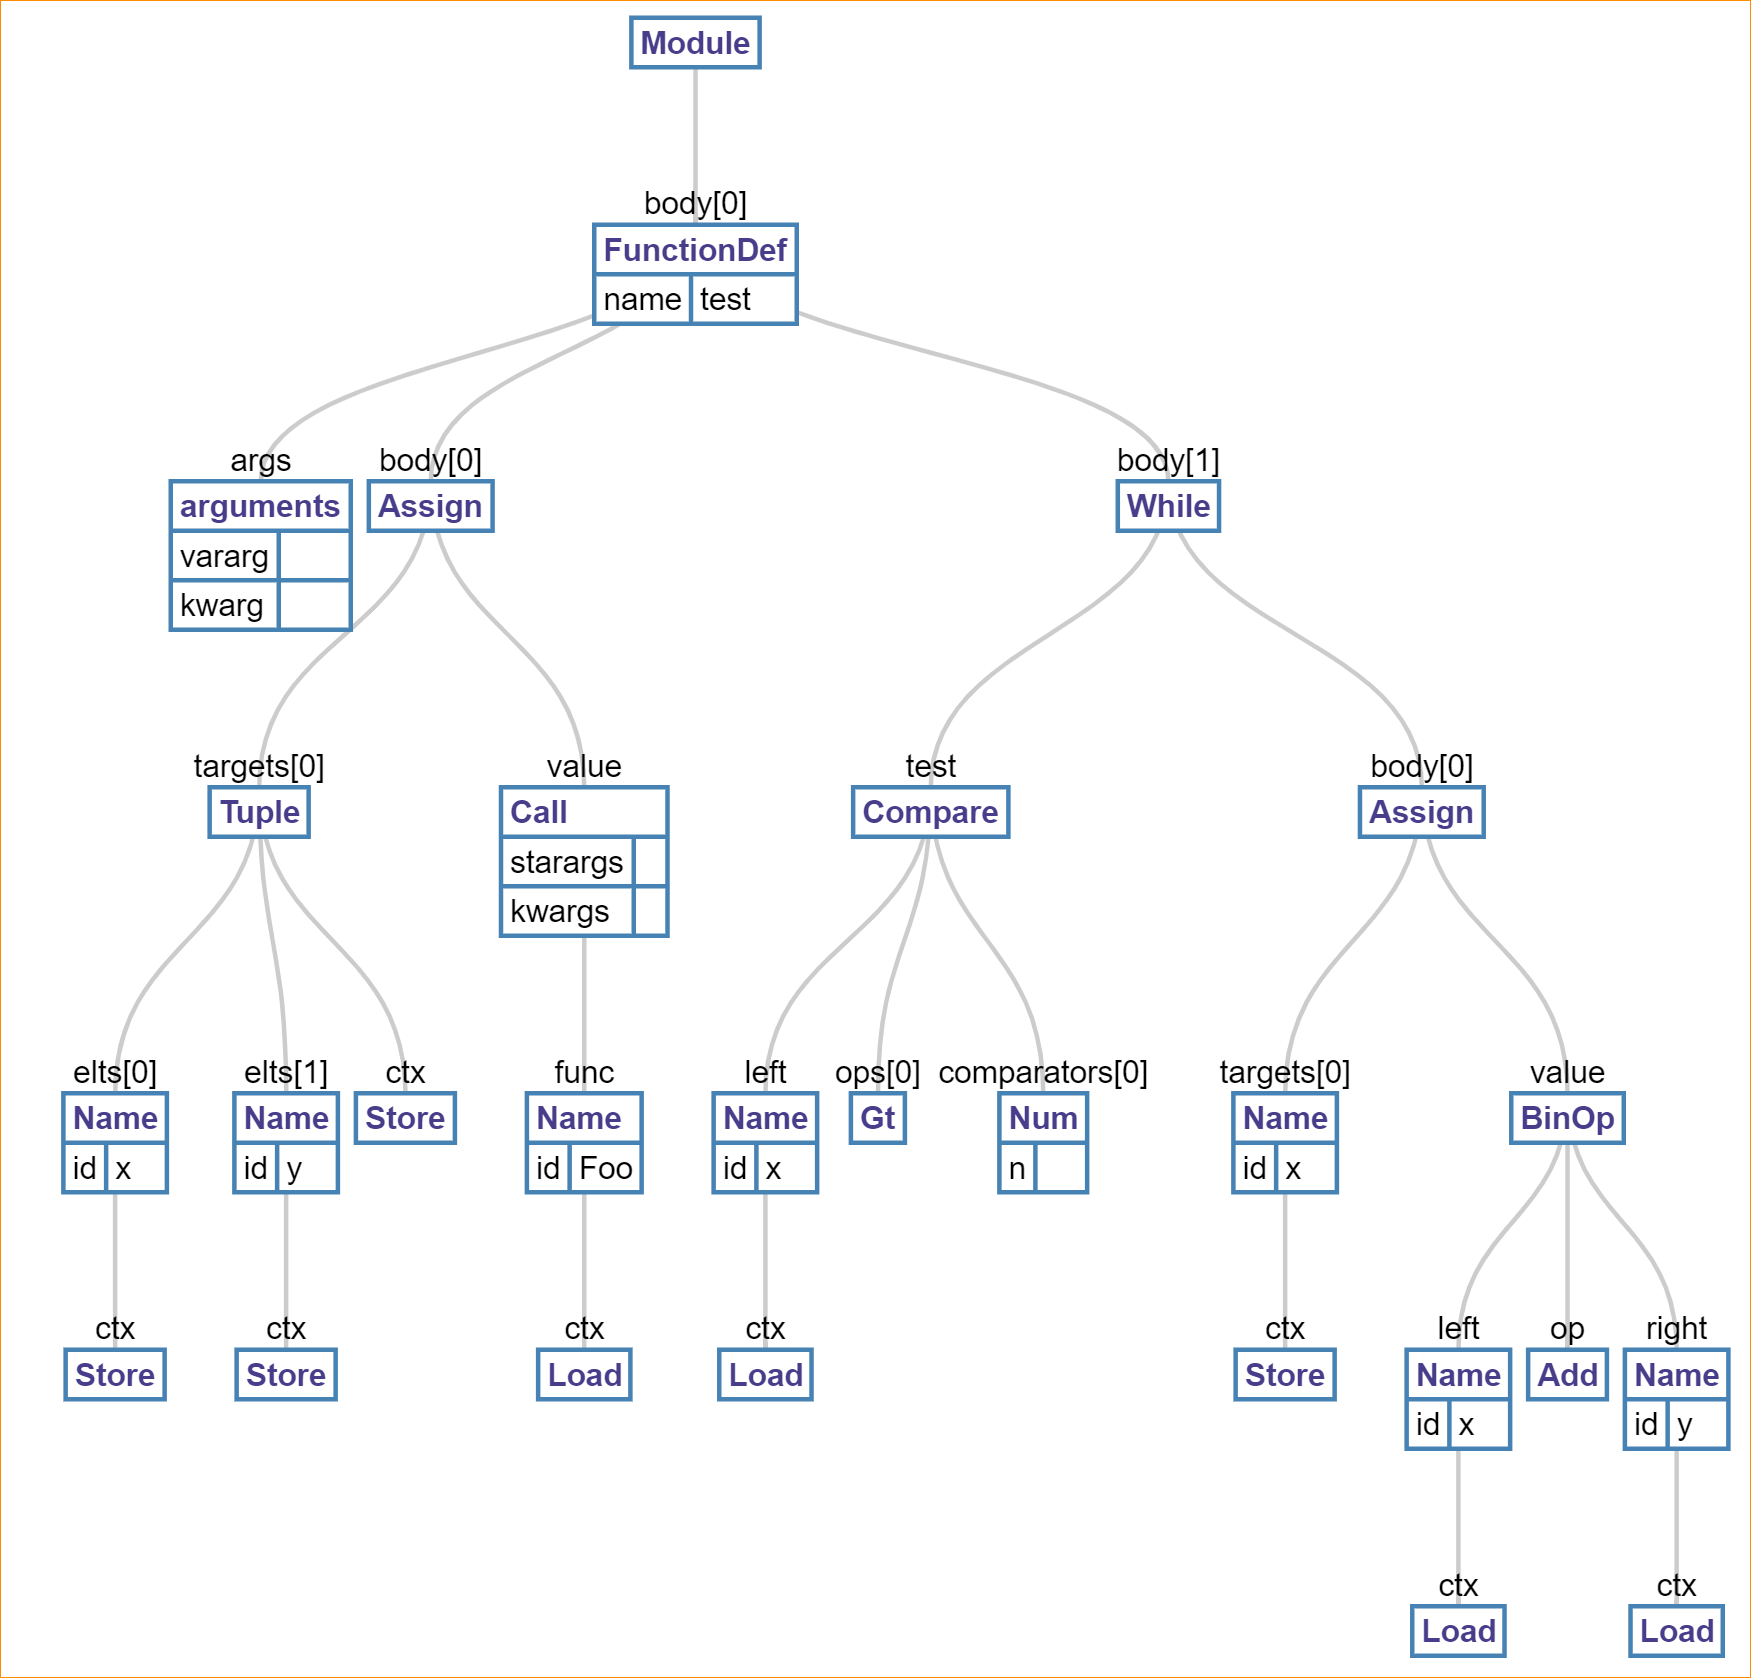
\includegraphics[width=0.5\textwidth,trim=4 4 4 4,clip]{AST2.png}
 \centering
 
    \begin{center}
    \begin{tabular}{c}
    \begin{lstlisting}[language=Python]
    def test():
        (x,y) = Foo()
        while x > 0:
            x = x + y

    \end{lstlisting}
    \end{tabular}
    \end{center}

\caption{\label{fig:ast}Sample function and the corresponding AST}
\end{figure}


\begin{figure}[h]
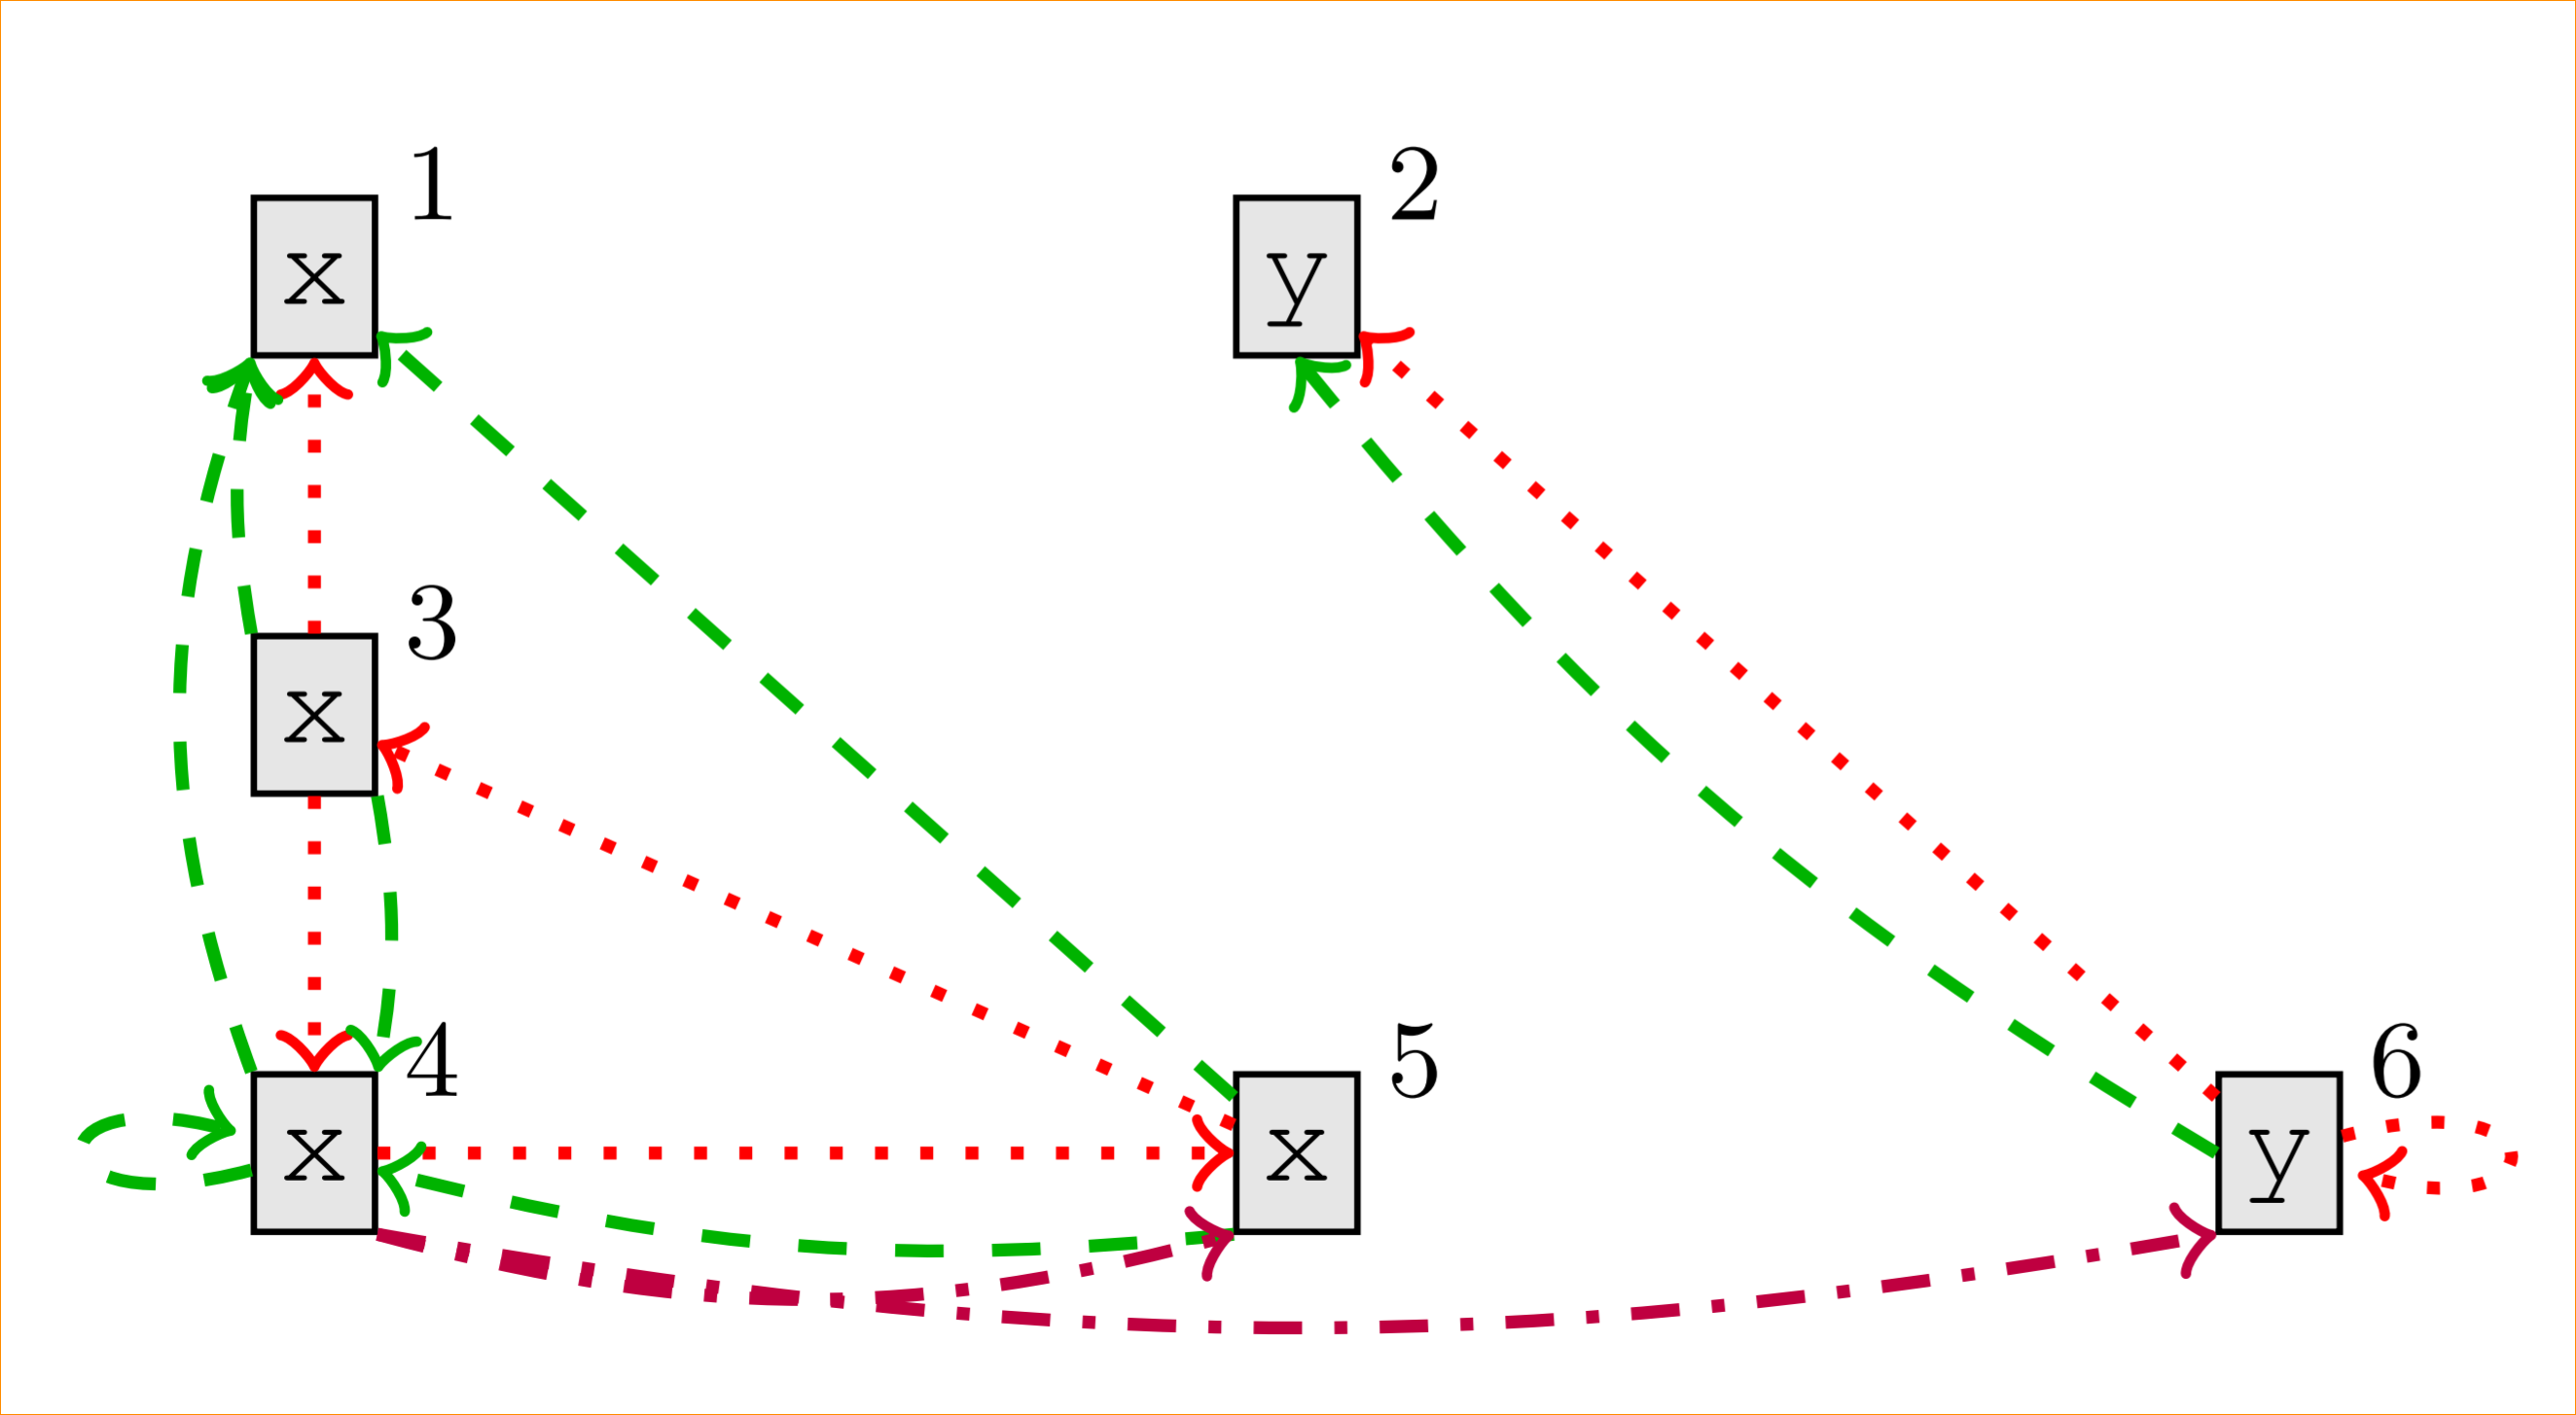
\includegraphics[width=0.5\textwidth,trim=4 4 4 4,clip]{data_flow.png}
 \centering
\caption{\label{fig:flow}Data flow edges for AST augmentation with red dotted LastUse edges, green dashed LastWrite edges and dash-dotted
purple ComputedFrom edges.\cite{1711.00740}.}
\end{figure}

\section{The CodeSearchNet Challenge}

Semantic code search is the task of retrieving relevant code given a natural language query. While related to other information retrieval tasks, it requires bridging the gap between the language used in code, often abbreviated and highly technical, and natural language more suitable to describe vague concepts and ideas.
The CodeSearchNet Challenge consists of 99 natural language queries with about 4k expert relevance annotations of likely results from CodeSearchNet Corpus. The corpus contains about 6 million functions from open-source code spanning six programming languages (Go, Java, JavaScript, PHP, Python, and Ruby). The CodeSearchNet Corpus also contains automatically generated query-like natural language for 2 million functions, obtained from mechanically scraping and preprocessing associated function documentation \cite{1909.09436}. 

Although the CodeSearchNet Corpus spans six different languages, this paper focuses only on the Python part, mainly because transforming each language code samples to graphs requires language-specific graph generators. For the Python Corpus, an existing open source Python 3 graph generator from \url{https://github.com/CoderPat/structured-neural-summarization/tree/master/parsers/sourcecode/barone} \cite{1811.01824} was reused and customized. Approximately $0.1\%$ of the original Python Corpus samples was removed because of syntactic errors, most probably written in Python 2. Based on baseline experiments run before and after the data reduction, the effect in the baseline accuracy was negligible.

\section{CodeSearchNet baseline models}

CodeSearchNet offers a range of baseline models for the code search task, using standard techniques from neural sequence processing. These baseline models use
\emph{joint embeddings}~\cite{gu2018deep,mitra2018introduction} of code and queries to implement a neural search
system. The architecture consists of two encoders, one encoder per language, natural or programming, and trains the encoders to map inputs into a single, joint vector
space.
The training objective is to map code and the corresponding natural language onto vectors that are near to each other, and use the query and code embedding vectors distance as a search ranking mechanism\cite{1909.09436} as depicted in \autoref{fig:model arch}.

\begin{figure}[t]
    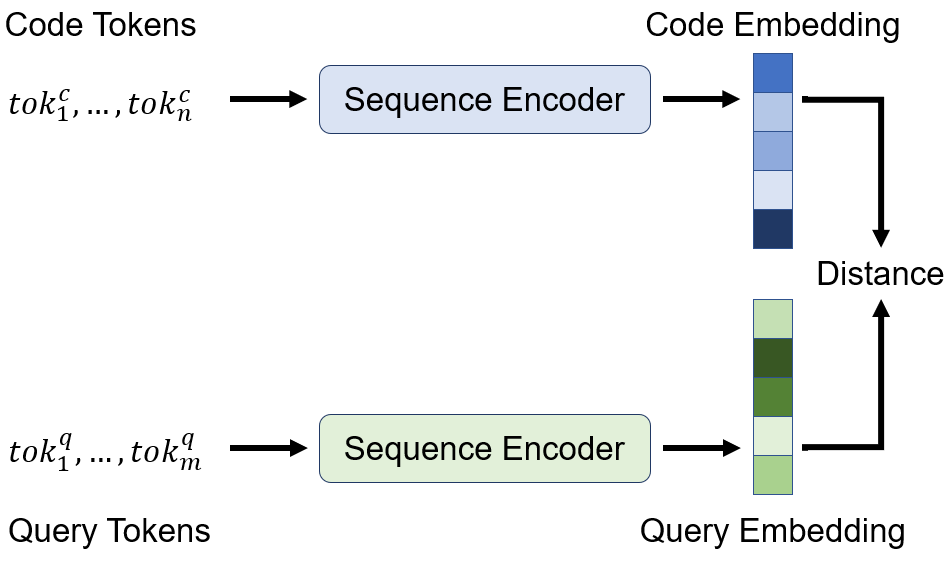
\includegraphics[width=\columnwidth]{ModelArchOverview.png}
    \caption{\label{fig:model arch}Baseline Model Architecture Overview\cite{1909.09436}.}
\end{figure}

The natural language tokens are split using byte-pair encoding (BPE)~\cite{gage1994new,sennrich2016neural}, and the Python language identifiers are split into sub-tokens ( i.e. a variable \texttt{camelCase} yields two sub-tokens \texttt{camel} and \texttt{case}). Then, the token sequences are processed to obtain (contextualized) token embeddings, using one of the following architectures.
\begin{description}
    \item[Neural Bag of Words] where each (sub)token is
      embedded to a learnable embedding (vector
      representation).
    \item[Bidirectional RNN models] the GRU cell~\cite{cho2014properties} is employed to summarize the input sequence.
    \item[1D Convolutional Neural Network] over the
      input sequence of tokens~\cite{kim2014convolutional}.
    \item[Self-Attention] where multi-head attention~\cite{vaswani2017attention}
      is used to compute representations of each token
      in the sequence.
    \item[Conv-Self-Att] a 1D-CNN+Self-Attention Hybrid.
\end{description}

The token embeddings are then combined into a sequence embedding using an attention-like weighted sum mechanism, with the final dimensionality of the embedding space set to \textbf{128}.
Given a set of $N$ pairs $(snippet_i, doc_i)$ of code and natural language descriptions, a code encoder $E_c$ and a query encoder $E_q$, the loss is defined as 

\begin{align*}
  -\frac{1}{N}\sum_i
        \log\left(\frac{\exp(E_c(c_i)^\top E_q(d_i))}
                       {\sum_ j \exp(E_c(c_j)^\top E_q(d_i))}\right)
\end{align*}

\section{Graph Neural Networks}

GNNs are a general neural network architecture defined according to a graph structure $G = (V, E)$. Nodes $v \in V$ take unique values from $1, . . . , |V|$, and edges are pairs $e = (v, v') \in V \times V$. 
The node vector (or node embedding) for node $v$ is denoted by $h_v \in R^D$. Graphs may also contain node labels $l_v \in \{1, . . . , L_V \}$ for each node $v$ and edge labels or edge types $l_e \in \{1, . . . , L_E \}$ for each edge. These edge labels are effectively the different syntactic and semantic node relationships, and since these relationships are directed, their reverse relationship equivalent.

Graph Neural Networks (GNNs) map graphs to outputs in two steps. First, there is a propagation step that computes node representations for each node, and second, an output model $o_v = g(h_v, l_v)$ maps from node representations and corresponding labels to an output $o_v$ for each $v \in V$. The system is differentiable from end-to-end, so all parameters are learned jointly using gradient-based optimization\cite{1511.05493}.

Many permutations of different GNNs exist. A homogeneous collection of a few popular GNNs TensorFlow implementation has been published at \url{https://github.com/microsoft/tf-gnn-samples} by the Deep Program Understanding team of  Microsoft Research, Cambridge, UK. 
These architectures are:
\begin{description}
    \item[Gated Graph Neural Networks] (GGNN)~\cite{1511.05493}.
    \item[Relational Graph Convolutional Networks] (RGCN)~\cite{1703.06103}.
    \item[Relational Graph Attention Networks] (RGAT) a generalization of Graph Attention Networks~\cite{1710.10903} to several edge types.
    \item[Graph Neural Network with Edge MLPs] (GNN-Edge-MLP) a variant of RGCN in which messages on edges are computed using full MLPs, not just a single layer.
    \item[Graph Neural Networks with Feature-wise Linear Modulation] (GNN-FiLM) a new extension of RGCN with FiLM layers~\cite{1709.07871}.
\end{description}

For the Graph Nodes tokenization, the Python code identifiers are split into sub-tokens using the PEP 8 standard naming conventions,  and each sub-token is further split into BPE sub-tokens using byte-pair encoding~\cite{gage1994new,sennrich2016neural}, similarly to the natural language tokenization. The usage of the additional BPE tokenization improved the accuracy for all different GNNs. The BPE sub-token embeddings are combined using a weighted sum pooling to produce the Graph Node embeddings, and the latter are combined into a sequence embedding using an attention-like weighted max-pooling mechanism. The attention layer contribution was a small, but nevertheless a notable increase of the total accuracy.
The training \textbf{batch size of 200 Graphs} was found to yield the best results.

For testing purposes on CodeSearchNet Corpus, a fixed set
of 999 distractor snippets $c_j$ for each test pair $(c_i
, d_i)$ was used, tested in all trained models . \autoref{tbl:mrr eval} presents the Mean Reciprocal Rank results on this task for the baseline and all used GNNs.

\subsection{GGNN Propagation Model}

The basic recurrence of the propagation model is

\begin{center}
\small
\begin{minipage}{.48\linewidth}
\begin{align}
    \noderept{\node}{1} & = [\labelsv_\node^\top, \mathbf{0}]^\top \label{eq:init}\\
    \nodeactt{\node}{t} & = 
    %[\noderept{\node_\out}{t}; \noderept{\node_\inc}{t}] = 
    \Av_{\node:}^\top  \left[\noderept{1}{t-1}{}^\top \ldots
\noderept{|\nodes|}{t-1}{}^\top\right]^\top + \bv \label{eq:propagate-A} \\
    \updategates_{\node}^{t} & =
    \sigma\left(\weights{}^{\updategate}\nodeactt{\node}{t} +
    \selfweights^{\updategate}\noderept{\node}{t-1}\right) \label{eq:update-gate}
\end{align}
\end{minipage}
\hfill
\begin{minipage}{.48\linewidth}
\begin{align}
    \resetgates_{\node}^{t} & =
    \sigma\left(\weights{}^{\resetgate}\nodeactt{\node}{t} +
    \selfweights^{\resetgate}\noderept{\node}{t-1}\right) \label{eq:reset-gate} \\
    \widetilde{\noderept{\node}{t}} & =
    \transform\left(\weights{}\nodeactt{\node}{t} +
    \selfweights\left(\resetgates_{\node}^{t}\odot\noderept{\node}{t-1}\right)\right)
    \\
    \noderept{\node}{t} & = (1 - \updategates_{\node}^{t})\odot
    \noderept{\node}{t-1} + \updategates_{\node}^{t}\odot
    \widetilde{\noderept{\node}{t}}.
\end{align}
\end{minipage}
\end{center}

The matrix $\Av \in \reals^{D|\nodes| \times 2 D |\nodes|}$ determines
how nodes in the graph communicate with each other. The sparsity
structure and parameter tying in $\Av$ is illustrated in
\figref{fig:graphs-and-sparsity}. The sparsity structure corresponds to the
edges of the graph, and the parameters in each
sub-matrix are determined by the edge type and direction.
$\Av_{\node:} \in \reals^{D|\nodes| \times 2 D}$ are the two columns of blocks
in $\Av^{(\mathrm{out})}$ and $\Av^{(\mathrm{in})}$ corresponding to node $\node$.
\eqref{eq:init} is the initialization step, which copies node annotations
into the first components of the hidden state and pads the rest with
zeros.  \eqref{eq:propagate-A} is the step that passes information
between different nodes of the graph via incoming and outgoing edges
with parameters dependent on the edge type and direction.
$\nodeactt{\node}{t}\in\reals^{2D}$ contains activations from edges in both
directions.
The remaining are GRU-like updates that incorporate information from the
other nodes and from the previous timestep to update each node's
hidden state.  $\updategates$ and $\resetgates$ are the update and
reset gates, $\sigma(x)=1/(1+e^{-x})$ is the logistic sigmoid
function, and $\odot$ is element-wise multiplication. %, and $\noderept{\node_\inc}{t}$ and
%$\noderept{\node_\out}{t}$ aggregate information from the incoming
%edges and outgoing edges respectively.

\begin{figure}[t]
\begin{center}
\begin{tabular}{ccc}
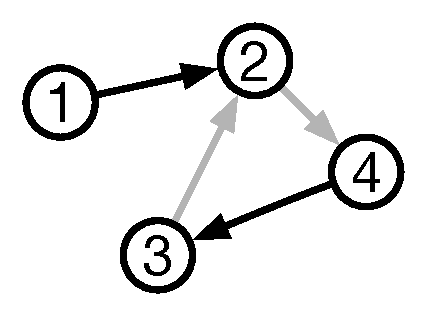
\includegraphics[width=.25 \columnwidth]{figs/example-graph.pdf} &
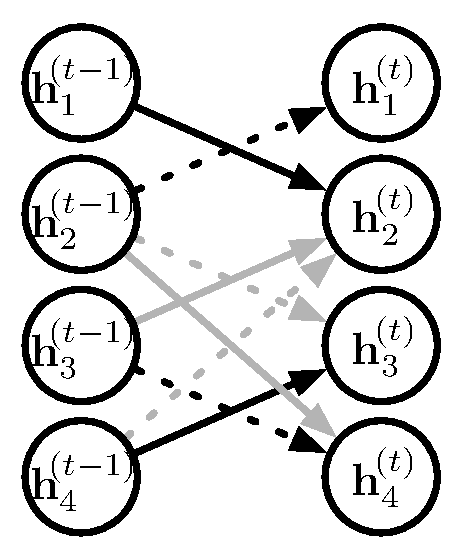
\includegraphics[width=.18 \columnwidth]{figs/unrolled-graph3.pdf} &
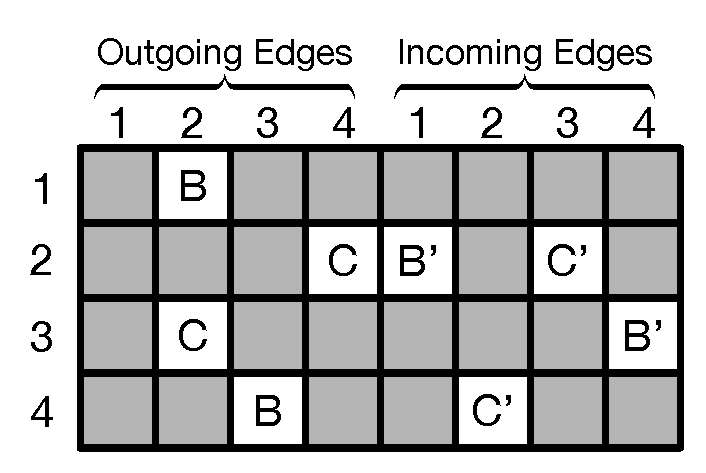
\includegraphics[width=.32 \columnwidth]{figs/recurrent-matrix-sparsity-pattern2.pdf}
\\
(a) & (b) & (c) $\Av = \left[ \Av^{(\hbox{\tiny{out}})},  \Av^{(\hbox{\tiny{in}})} \right]$
\end{tabular}
\end{center}
\vspace{-10pt}
\caption{
  (a) Example graph. Color denotes edge types.
  (b) Unrolled one timestep.
  (c) Parameter tying and sparsity in recurrent matrix. Letters denote
  edge types with $B'$ corresponding to the reverse edge of type $B$.
  $B$ and $B'$ denote distinct parameters.
}
\label{fig:graphs-and-sparsity}
\end{figure}

\begin{table*}[t]
  \begin{tabular}{@{}llllll@{}} \toprule
  \multicolumn{2}{c}{Encoder}&&\multicolumn{2}{c}{MRR}&\\\midrule
  
  \multicolumn{1}{c}{Text} & \multicolumn{1}{c}{Code} && \multicolumn{1}{c}{Validation} & \multicolumn{1}{c}{Test} &  \\ \midrule
  
  SelfAtt (BERT) & SelfAtt (BERT) && \textbf{0.5800} & \textbf{0.6505} \\
  ConvSelfAtt & ConvSelfAtt && 0.5604 & 0.5822 \\ 
  NBoW & NBoW && 0.4708 & 0.6387 \\
  1D-CNN & 1D-CNN && 0.4753 & 0.5465 \\
  biRNN & biRNN && 0.5078 & 0.6404\\\midrule
  ConvSelfAtt & GGNN && \textbf{0.5358} & \textbf{0.5175} \\
  ConvSelfAtt & RGAT && 0.4431 & 0.3946 \\
  ConvSelfAtt & GNN-FiLM && 0.4896 & 0.3036 \\
  ConvSelfAtt & GNN Edge-MLP && 0.506 & 0.3024 \\
  ConvSelfAtt & RGCN && 0.4147 & 0.2410 \\

  \bottomrule
  \end{tabular}
  \caption{Mean Reciprocal Rank (MRR) on Validation and Test Sets of CodeSearchNet Python corpus. As a test, the models try to rank the correct code snippet highly among 999 distractor snippets.} \label{tbl:mrr eval}
\end{table*}

\section{Results}

As reflected in the \autoref{tbl:mrr eval}, GGNN was the best performing GNN. For this reason the formal definition of the GGNN propagation model is repeated here for convenience, as it was originally described in \cite{1511.05493}. 

A notable discrepancy exists between the test and validation results. While the MRR decreases in the test results, the MRR increases for the baseline. One possible reason due to the way the data were stratified by the CodeSearchNet competition organizers. Indeed, it seems that the data were not shuffled but stratified by keeping the order that were collected. The competition Corpus is effectively a collection of the most popular Python GitHub repositories, possibly starting from the most popular repositories and continuing in a descending order. One indication of this is the fact that the validation loss increases monotonically during the validation steps of each epoch. This means that as the repositories become less popular, the code "quality" drops, in other words, the noise level increases.
Also, when plotting the samples loss, as stratified, there is a clear indication of clusters with similar loss. This could be explained by the fact that the individual samples are functions extracted from each repository and, most probably, the neighbouring functions come from the same repositories that share similar noise levels.
Based on these assumptions, we can see that the GNNs are more sensitive to the code quality, possibly because better code means much simpler graphs.

This possible issue was reported to the CodeSearchNet repository here:  \url{https://github.com/github/CodeSearchNet/issues/87}

\section{Conclusions}
Overall, the GNN models achieved somewhat good performance on this task, but failed to exceed the BERT-based models which had the best performance. This is not unexpected, as the self-attention model has the highest capacity of all considered models. GGNN had a notable performance, since it was the best performing GNN and for the validation dataset, very close to the top performers, making it a very promising alternative to BERT. Nevertheless, more work is needed around the GNNs sensitivity to noisy data.

Two samples can be found in the Appendices, one with rank 1 \autoref{appendix:good}, and one with the rank 919 \autoref{appendix:bad}. An obvious difference is the fact that the code comment (docstring) of the latter is more elaborate and complex. This complexity has an obvious negative effect in the whey the GNNs encode the information and as an effect, to the final ranking.

\section{Future improvements}
Possible future improvements are: 
\begin{itemize}
  \item Better hyper-parameters tuning. Due to time constraints, not all hyper-parameter combinations where thoroughly explored.
  \item Better data shuffling between the data strata.
  \item A richer semantic graph enhancement, by leveraging more static code analysis heuristics. For example, metadata of the identifiers type could be added to the graph nodes.
  \item Combine the Natural Language information included in the code comments, with a traditional NLP model as a hybrid.
  \item Include docstring parsers that parse the comments and provide information that can be mapped in the code graph, for example, as metadata of the parameters.
\end{itemize}


\section*{Acknowledgements}
The author would like to thank Miltiadis Allamanis, Senior Researcher at Microsoft Research in Cambridge, UK, for his valuable guidance.

\bibliographystyle{unsrt}  
\bibliography{references} 




\begin{appendices}


\section{Rank 1 sample}
\label{appendix:good}
\begin{lstlisting}[language=Python, caption={Sample that ranked first},captionpos=b]
def get_feature_counts(self, threshold=0.001):
     """ Returns a dictionary, where the keys are the feature names
     and the values are the number of studies tagged with the feature. """
     counts = np.sum(self.get_feature_data() >= threshold, 0)
     return dict(zip(self.get_feature_names(), list(counts)))
\end{lstlisting}

\section{Rank 919 sample}
\label{appendix:bad}
\begin{lstlisting}[language=Python, caption={Sample that ranked first},captionpos=b]
def gsea(data, gene_sets, cls, outdir='GSEA_', min_size=15, max_size=500, permutation_num=1000,
    weighted_score_type=1,permutation_type='gene_set', method='log2_ratio_of_classes',
     ascending=False, processes=1, figsize=(6.5,6), format='pdf',
    graph_num=20, no_plot=False, seed=None, verbose=False):
    """ Run Gene Set Enrichment Analysis.
    
    :param data: Gene expression data table, Pandas DataFrame, gct file.
    :param gene_sets: Enrichr Library name or .gmt gene sets file or dict of gene sets. Same input with GSEA.
    :param cls: A list or a .cls file format required for GSEA.
    :param str outdir: Results output directory.
    :param int permutation_num: Number of permutations for significance computation. Default: 1000.
    :param str permutation_type: Permutation type, \"phenotype\" for phenotypes, \"gene_set\" for genes.
    :param int min_size: Minimum allowed number of genes from gene set also the data set. Default: 15.
    :param int max_size: Maximum allowed number of genes from gene set also the data set. Default: 500.
    :param float weighted_score_type: Refer to :func:`algorithm.enrichment_score`. Default:1.
    :param method: The method used to calculate a correlation or ranking. Default: 'log2_ratio_of_classes'.
    Others methods are:
    
    1. 'signal_to_noise'
    
    You must have at least three samples for each phenotype to use this metric.
    The larger the signal-to-noise ratio, the larger the differences of the means (scaled by the standard deviations);
    that is, the more distinct the gene expression is in each phenotype and the more the gene acts as a “class marker.”
    
    2. 't_test'
    
    Uses the difference of means scaled by the standard deviation and number of samples.
    Note: You must have at least three samples for each phenotype to use this metric.
    The larger the tTest ratio, the more distinct the gene expression is in each phenotype
    and the more the gene acts as a “class marker.”
    
    3. 'ratio_of_classes' (also referred to as fold change).
    
    Uses the ratio of class means to calculate fold change for natural scale data.
    
    4. 'diff_of_classes'
    
    
    Uses the difference of class means to calculate fold change for nature scale data
    
    
    5. 'log2_ratio_of_classes'
    
    Uses the log2 ratio of class means to calculate fold change for natural scale data.
    This is the recommended statistic for calculating fold change for log scale data.
    
    
    :param bool ascending: Sorting order of rankings. Default: False.
    :param int processes: Number of Processes you are going to use. Default: 1.
    :param list figsize: Matplotlib figsize, accept a tuple or list, e.g. [width,height]. Default: [6.5,6].
    :param str format: Matplotlib figure format. Default: 'pdf'.
    :param int graph_num: Plot graphs for top sets of each phenotype.
    :param bool no_plot: If equals to True, no figure will be drawn. Default: False.
    :param seed: Random seed. expect an integer. Default:None.
    :param bool verbose: Bool, increase output verbosity, print out progress of your job, Default: False.
    
    :return: Return a GSEA obj. All results store to a dictionary, obj.results,
    where contains::
    
    | {es: enrichment score,
    | nes: normalized enrichment score,
    | p: P-value,
    | fdr: FDR,
    | size: gene set size,
    | matched_size: genes matched to the data,
    | genes: gene names from the data set
    | ledge_genes: leading edge genes}
    
    
    """
    gs = GSEA(data, gene_sets, cls, outdir, min_size, max_size, permutation_num,
    weighted_score_type, permutation_type, method, ascending, processes,
    figsize, format, graph_num, no_plot, seed, verbose)
    gs.run()
    
    return gs

\end{lstlisting}

\end{appendices}
\end{document}
